\setchaptergraphic{
    % Petersen graph
    \newcommand*{\radius}{3.0}
    \pgfmathsetmacro{\inner}{\radius*0.5*(sqrt(5)-1)}
    \begin{tikzpicture}
        \begin{scope}[every node/.style={circle,thick,draw,fill=cyan}]
            \node (a1) at ({\radius*cos(90)}, {\radius*sin(90)}) {};
            \node (a2) at ({\inner*cos(90+90)}, {\inner*sin(90+90)}) {};
            \node (b1) at ({\radius*cos(162)}, {\radius*sin(162)}) {};
            \node (b2) at ({\inner*cos(162+90)}, {\inner*sin(162+90)}) {};
            \node (c1) at ({\radius*cos(234)}, {\radius*sin(234)}) {};
            \node (c2) at ({\inner*cos(234+90)}, {\inner*sin(234+90)}) {};
            \node (d1) at ({\radius*cos(306)}, {\radius*sin(306)}) {};
            \node (d2) at ({\inner*cos(306+90)}, {\inner*sin(306+90)}) {};
            \node (e1) at ({\radius*cos(18)}, {\radius*sin(18)}) {};
            \node (e2) at ({\inner*cos(18+90)}, {\inner*sin(18+90)}) {};
        \end{scope}

        \begin{scope}[>={Stealth[black]},
                    every node/.style={fill=white,circle},
                    every edge/.style={draw=black,very thick}]
            \path [-] (a1) edge (a2);
            \path [-] (b1) edge (b2);
            \path [-] (c1) edge (c2);
            \path [-] (d1) edge (d2);
            \path [-] (e1) edge (e2);

            \path [-] (a1) edge (b1);
            \path [-] (b1) edge (c1);
            \path [-] (c1) edge (d1);
            \path [-] (d1) edge (e1);
            \path [-] (e1) edge (a1);

            \path [-] (a2) edge (c2);
            \path [-] (c2) edge (e2);
            \path [-] (e2) edge (b2);
            \path [-] (b2) edge (d2);
            \path [-] (d2) edge (a2);
        \end{scope}
    \end{tikzpicture}
}

\chapter{Graph Theory}
\label{ch:graph}

\section{Graphs}

\begin{defn}
    A \emph{simple graph} is a $2$-tuple $G = (V, E)$, where $V$ is a non-empty finite set of vertices, and $E$ is a set of unordered pairs (two-sets) of distinct vertices, called edges.
\end{defn}

\begin{rmk}
    We may also write $V$ as $V(G)$, and $E$ as $E(G)$.
\end{rmk}

\begin{exmp}
    Let $G = \left(\left\{a, b, c, d\right\}, \left\{\{a, b\}, \{a, c\}, \{b, d\}\right\}\right)$. This graph is depicted in Figure \ref{fig:example-simple-graph}.
\end{exmp}

\begin{figure}[ht!]
    \centering
    \begin{tikzpicture}
        \begin{scope}[every node/.style={circle,thick,draw,fill=cyan}]
            \node (a) at (0,0) {a};
            \node (b) at (3,1.5) {b};
            \node (c) at (3,-1.5) {c};
            \node (d) at (6,0) {d};
        \end{scope}

        \begin{scope}[>={Stealth[black]},
                    every node/.style={fill=white,circle},
                    every edge/.style={draw=black,very thick}]
            \path [->] (a) edge (b);
            \path [->] (a) edge (c);
            \path [->] (b) edge (d);
        \end{scope}
    \end{tikzpicture}
\caption{Example simple graph}
\label{fig:example-simple-graph}
\end{figure}

\begin{defn}
    Let $G = (V, E)$ be a graph. If $u, v \in V$, then we say $u$ is \emph{adjacent to} $v$ when $\{u, v\} \in E$. We denote this by $u \sim v$, and say that $u$ and $v$ are the endpoints of the edge $\{u, v\}$. We further say that $u$ or $b$ is \emph{incident on} or \emph{incident with} $\{u, v\}$.
\end{defn}

\begin{defn}
    Let $G = (V, E)$ be a graph. If $u, v \in V$ are adjacent, then we say $u$ and $v$ are \emph{neighbors}. The set of all neighbors of $v$ is the \emph{neighborhood} of $v$:
    \[N(v) = \left\{u \in V \compbar u \sim v \right\}.\]
\end{defn}

\begin{defn}
    A \emph{graph isomorphism} between graphs $G$ and $H$ is a pair of bijections $(\theta, \varphi)$ where $\theta: V(G) \to V(H)$ and $\varphi: E(G) \to E(H)$ such that vertex $v$ is indicent with edge $e$ in $G$ \emph{if and only if} vertex $\theta(v)$ is incident with edge $\varphi(e)$ in $H$.
\end{defn}

\begin{figure}[ht!]
    \centering
    \begin{tikzpicture}
        \begin{scope}[every node/.style={circle,thick,draw,fill=cyan}]
            \node (1) at ({2*cos(180)}, {2*sin(180)}) {1};
            \node (2) at (0, 0) {2};
            \node (3) at ({3*cos(60)}, {2*sin(60)}) {3};
            \node (4) at ({3*cos(300)}, {2*sin(300)}) {4};
        \end{scope}

        \begin{scope}[>={Stealth[black]},
                    every node/.style={fill=white,circle},
                    every edge/.style={draw=black,very thick}]
            \path [-] (1) edge["1"] (2);
            \path [-] (1) edge["2"] (3);
            \path [-] (2) edge["3"] (3);
            \path [-] (2) edge["4"] (4);
            \path [-] (3) edge["5"] (4);
        \end{scope}
    \end{tikzpicture}
\caption{Example graph}
\label{fig:adjacency-example}
\end{figure}

\begin{defn}
    The \emph{adjacency matrix} $A(G)$ of a graph $G = (V, E)$ is a square $|V| \times |V|$ matrix where $A(G)_{i, j}$ is $1$ if there is an edge from $V_i$ to $V_j$, and $0$ otherwise.
\end{defn}

\begin{exmp}
    The adjacency matrix of the graph shown in Figure \ref{fig:adjacency-example} is
    \[A = \begin{bmatrix}
        0 & 1 & 1 & 1 \\
        1 & 0 & 1 & 0 \\
        1 & 1 & 0 & 1 \\
        1 & 0 & 1 & 0
    \end{bmatrix}.\]
\end{exmp}

\begin{rmk}
    The adjacency matrix of a simple graph clearly must be symmetric and have only zeroes on the major diagonal (since simple graphs do not have loop edges).
\end{rmk}

\begin{defn}
    Let $G = (V, E)$ be a graph, and $\textrm{lex}: E \to \Z_n$ be an order of edges. The \emph{incidence matrix} $B(G)$ of a graph $G = (V, E)$ is a $\abs{V(G)}$ by $\abs{E(G)}$ rectangular matrix, such that
    \begin{align*}
        B_{v, \textrm{lex}(e)} = \begin{dcases}
            1, &e \textrm{ is incident to v}, \\
            0, &\textrm{otherwise}
        \end{dcases}.
    \end{align*}
\end{defn}

\begin{exmp}
    The incidence matrix of the graph shown in Figure \ref{fig:adjacency-example}, using $\textrm{lex}(e_i) = i$, is
    \begin{align*}
        B = \begin{bmatrix}
            1 & 1 & 0 & 0 & 0 \\
            1 & 0 & 1 & 1 & 0 \\
            0 & 1 & 1 & 0 & 1 \\
            0 & 0 & 0 & 1 & 1 \\
        \end{bmatrix}.
    \end{align*}
\end{exmp}

\begin{defn}
    Let $G = (V, E)$ be a graph. The \emph{Sylvester adjacency polynomial} of $G$ is the polynomial in variables $x_i$ given by
    \begin{align*}
        \prod_{\substack{i < j \\ i \textrm{ adjacent to } j}}\left(x_j-x_i\right).
    \end{align*}
\end{defn}

\begin{defn}
    Edge list monomial
    \begin{align*}
        \prod_{i \textrm{ adjacent to } j}y_{i, j}
    \end{align*}
\end{defn}

\begin{defn}
    Let $G$ be a graph. The \emph{degree} of a vertex $v \in V$, denoted by $d_G(v)$, is the number of edges with which $v$ is incident. In a simple graph, it is the number of neighbors of $v$. \[d_G(v) = |N(v)|.\]
\end{defn}

\begin{prop}\label{adjacency-sum}
    Let $G = (V, E)$ be a graph, and $\bm{A}$ its adjacency matrix. The sum of all entries of $\bm{A}$ is the sum of the degrees of all vertices in $G$.
\end{prop}

\begin{proof}
    The sum of entries in the $i$th row of $\bm{A}$ is the degree of $V_i$, since there is a single $1$ for every vertex $V_i$ is adjacent to. Therefore, the sum of the sum of each row gives the sum of degrees of vertices in $G$.
\end{proof}

\begin{thm}{Handshake Lemma}\label{sum-degrees-is-twice-edges}\proofbreak
    Let $G = (V, E)$ be a graph. The sum of the degrees of all vertices in $G$ is twice the number of edges:
    \[\sum_{v\in V}d_G(v) = 2|E|.\]
\end{thm}

\begin{proof}
    By Proposition \ref{adjacency-sum}, we know that this sum is equal to the sum of the adjacency matrix of $G$. Since the adjacency matrix is symmetric, and has all zero entries on the major diagonal, its sum must be an even number equal to twice the sum of entries above the major diagonal (the upper triangular region).

    We must then show that the sum of entries above the major diagonal is equal to the number of edges in $G$. Every edge can of course be represented uniquely as $(V_i, V_j)$, where $j > i$, which is precisely the sum of entries above the major diagonal in the adjacency matrix.
\end{proof}

\begin{cor}\label{n-of-odd-vertices-is-even}
    The number of vertices with odd degree is even.
\end{cor}

\begin{proof}
    For the sake of contradiction, assume that a graph $G$ has an odd number of vertices with odd degree. Then, the sum of degrees of vertices with even degree must itself be even, and the sum of degrees of vertices with odd degree must be odd, so the sum of the degrees of all vertices in $G$ is odd. By Corollary \ref{sum-degrees-is-twice-edges}, this is a contradiction.
\end{proof}

\begin{thm}
    Let $G, H$ be graphs such that $V(G) = V(H)$, and let $n = \abs{V(G)}$. Then $G$ are $H$ are isomorphic if and only if there exists a solution $P \in \C^{n\times n}$ to the system
    \begin{align*}
        PA(G)P^{*} &= A(H), \\
        PP^{*} &= I, \\
        P \circ P &= P,
    \end{align*}
    where $\circ$ is the Hadamard product.
\end{thm}

\begin{proof}
    Suppose we have solved a relaxed version of this problem, by finding $R \in C^{n \times n}$ such that $RA(G)R^{*} = A(H)$ and $RR^{*} = I$. Then $A(G)$ and $A(H)$ must have the same eigenvalues. Let $D$ be a diagonal matrix of these eigenvalues. Since $A(G)$ and $A(H)$ are real symmetric matrices, by the Spectral Theorem \ref{spectral-theorem}, there exists eigendecompositions $A(G) = UD\transposeof{U}$ and $A(H) = VD\transposeof{V}$. Then $A_G = \left(U\transposeof{V}\right)A_H\transposeof{\left(U\transposeof{V}\right)}$.

    For $k \in \left\{0, 1\right\}$
    $\left(PA(G)^{k}P^{*}\right) \circ A(H)^{\circ^k} = A(H)^{k}$
\end{proof}

\begin{defn}
    An \emph{Eulerian trail} is a trail through a graph that visits every edge exactly once.
\end{defn}

\begin{defn}
    An \emph{Eulerian circuit} is an Eulerian trail that starts and ends on the same vertex.
\end{defn}

\begin{defn}
    A \emph{Hamiltonian path} is a path through a graph that visits every vertex exactly once.
\end{defn}

\begin{defn}
    A \emph{Hamiltonian cycle} is a Hamiltonian path that starts and ends with the same vertex.
\end{defn}

\begin{defn}
    Let $G = (V, E)$ be a graph. Then
    \[\Delta G = \max_{v \in V}d_G(v),\]
    \[\delta G = \min_{v \in V}d_G(v)\] are the maximum and minimum of all degrees of the vertices in $G$ respectively.
\end{defn}

\begin{defn}
    Let $G$ be a graph. Then the \emph{order} of $G$ is $|V(G)|$, and the \emph{size} of $G$ is $|E(G)|$.
\end{defn}

\begin{defn}
    A \emph{regular} graph is a simple graph is which every vertex has the same degree, so for every regular graph $G$, we have $\Delta G = \delta G$. If every vertex has degree $n$, it is an $n$-regular graph.
\end{defn}

\begin{defn}
    A \emph{complete} graph is one where every pair of vertices are adjacent. The unique complete graph with order $n$ is denoted by $K_n$.
\end{defn}

\begin{rmk}
    The graph $K_n$ has size $\binom{n}{2}$.
\end{rmk}

\begin{figure}[ht!]
    \centering
    \begin{tikzpicture}
        \begin{scope}[every node/.style={circle,thick,draw,fill=cyan}]
            \node (a) at ({4*cos(0)}, {4*sin(0)}) {};
            \node (b) at ({4*cos(60)}, {4*sin(60)}) {};
            \node (c) at ({4*cos(120)}, {4*sin(120)}) {};
            \node (d) at ({4*cos(180)}, {4*sin(180)}) {};
            \node (e) at ({4*cos(240)}, {4*sin(240)}) {};
            \node (f) at ({4*cos(300)}, {4*sin(300)}) {};
        \end{scope}

        \begin{scope}[>={Stealth[black]},
                    every node/.style={fill=white,circle},
                    every edge/.style={draw=black,very thick}]
            \path [-] (a) edge (b);
            \path [-] (a) edge (c);
            \path [-] (a) edge (d);
            \path [-] (a) edge (e);
            \path [-] (a) edge (f);

            \path [-] (b) edge (c);
            \path [-] (b) edge (d);
            \path [-] (b) edge (e);
            \path [-] (b) edge (f);

            \path [-] (c) edge (d);
            \path [-] (c) edge (e);
            \path [-] (c) edge (f);

            \path [-] (d) edge (e);
            \path [-] (d) edge (f);

            \path [-] (e) edge (f);
        \end{scope}
    \end{tikzpicture}
\caption{Depiction of $K_6$}
\label{fig:k-six}
\end{figure}

\begin{prop}
    Every complete graph is a regular graph.
\end{prop}

\begin{proof}
    Every vertex in $K_n$ is adjacent to exactly $n-1$ other vertices.
\end{proof}

\begin{defn}
    Let $H$ be a graph. We call a graph $G$ a \emph{subgraph} of $H$ provided that
    \begin{itemize}
        \item $V(G) \subseteq V(H)$,
        \item and $E(G) \subseteq E(H)$.
    \end{itemize}
\end{defn}

\begin{rmk}
    Every graph $G$ is a subgraph of itself.
\end{rmk}

\begin{defn}
    Let $H$ be a graph, and let $G$ be a subgraph of $H$. $G$ is a \emph{spanning} subgraph of $H$ provided that
    \begin{itemize}
        \item $V(G) = V(H)$,
        \item and $E(G) \subseteq E(H)$.
    \end{itemize}
\end{defn}

\begin{defn}
    Let $G$ be a graph, and let $e \in E(G)$. Then we denote by $G - e$ the spanning subgraph of $G$ given by \[G - e = (V(G), E(G) - \{e\}).\]
\end{defn}

\begin{defn}
    Let $H$ be a graph, and let $A \subseteq V(H)$. The subgraph of $H$ \emph{induced on} $A$ is the graph $H[A]$ with
    \begin{itemize}
        \item $V(H[A]) = A$,
        \item and $E(H[A]) = \left\{\{a, b\} \in E(H) \compbar a \in A \land b \in A\right\}$.
    \end{itemize}
\end{defn}

\begin{defn}
    Let $G$ be a graph, and let $v \in V(G)$. Then we denote by $G - v$ the subgraph of $G$ induced by $V(G) - v$, given by \[G - v = G[V(G) - \{v\}].\]
\end{defn}

\begin{figure}[ht!]
    \centering
    \begin{tikzpicture}
        \begin{scope}[every node/.style={circle,thick,draw,fill=cyan}]
            \node (1) at ({2*cos(180)}, {2*sin(180)}) {1};
            \node (2) at (0, 0) {2};
            \node (3) at ({3*cos(60)}, {2*sin(60)}) {3};
            \node (4) at ({3*cos(300)}, {2*sin(300)}) {4};
        \end{scope}

        \begin{scope}[>={Stealth[black]},
                    every node/.style={fill=white,circle},
                    every edge/.style={draw=black,very thick}]
            \path [-] (1) edge (2);
            \path [-] (2) edge (3);
            \path [-] (2) edge (4);
            \path [-] (3) edge (4);
        \end{scope}
    \end{tikzpicture}
\caption{Example graph}
\label{fig:clique-examples}
\end{figure}

\begin{defn}
    Let $G$ be a graph, and $S \subseteq V(G)$. If $u \sim v$ for all distinct $u, v \in S$, then we say that $S$ is a \emph{clique} in $G$.
\end{defn}

\begin{exmp}
    The following are all cliques in the graph depicted in Figure \ref{fig:clique-examples}:
    \begin{multicols}{2}
        \begin{itemize}
            \item $\emptyset$,
            \item $\{1\}$,
            \item $\{2\}$,
            \item $\{3\}$,
            \item $\{4\}$,
        \end{itemize}
        \columnbreak
        \begin{itemize}
            \item $\{1, 2\}$,
            \item $\{2, 3\}$,
            \item $\{2, 4\}$,
            \item $\{3, 4\}$,
            \item $\{2, 3, 4\}$.
        \end{itemize}
    \end{multicols}
\end{exmp}

\begin{defn}
    Let $G$ be a graph. The clique number of $G$, denoted by $\omega(G)$, is the maximum cardinality of all cliques in $G$.
\end{defn}

\begin{exmp}
    In the graph depicted in Figure \ref{fig:clique-examples}, the clique with maximum cardinality is $\{2, 3, 4\}$, so $\omega(G) = 3$.
\end{exmp}

\begin{defn}
    Let $G$ be a graph, and let $S$ be a clique in $G$.
    \begin{itemize}
        \item We say $S$ is \emph{maximum} if $|S| = \omega(G)$.
        \item We say $S$ is \emph{maximal} if it cannot be made larger by adding vertices to it.
    \end{itemize}
\end{defn}

\begin{exmp}
    In the graph depicted in Figure \ref{fig:clique-examples}, the only maximum clique is $\{2, 3, 4\}$, but both $\{1, 2\}$ and $\{2, 3, 4\}$ are maximal cliques.
\end{exmp}

\begin{defn}
    Let $G$ be a graph, and $S \subseteq V(G)$. If $u \not\sim v$ for all $u, v \in S$, then we say that $S$ is an \emph{independent set} in $G$.
\end{defn}

\begin{exmp}
    The following are all independent sets in the graph depicted in Figure \ref{fig:clique-examples}: $\emptyset$, $\{1\}$, $\{2\}$, $\{3\}$, $\{4\}$, $\{1, 3\}$, and $\{1, 4\}$.
\end{exmp}

\begin{defn}
    Let $G$ be a graph. The independence number of $G$, denoted by $\alpha(G)$, is the maximum cardinality of all independent sets in $G$.
\end{defn}

\begin{exmp}
    In the graph depicted in Figure \ref{fig:clique-examples}, an independent set with maximum cardinality is $\{1, 3\}$, so $\alpha(G) = 2$.
\end{exmp}

\begin{defn}
    A subset $S \subseteq V(G)$ is a \emph{vertex cover} of $G$ when every edge in $E(G)$ is adjacent to at least one vertex in $S$.
\end{defn}

\begin{prop}
    A subset $S \subseteq V(G)$ is an independent set if and only if $V(G)\setminus S$ is a vertex cover.
\end{prop}

\begin{proof}
    If $S$ is independent, then at most one of $u, v$ are in $S$ whenever $(u, v) \in E(G)$. Therefore, at least one of $u, v$ are in $V(G) \setminus S$.

    If $V(G)\setminus S$ is a vertex cover, then for every edge $(u, v) \in E(G)$, at least one of $u, v$ is in $V(G)\setminus S$. Therefore, at most one of $u, v$ is in $S$, and so $S$ must be an independent set.
\end{proof}

\begin{defn}Complement Graph\proofbreak
    Let $G$ be a graph. The \emph{complement graph} of $G$, denoted by $\bar{G}$, is defined by
    \[V(\bar{G}) = V(G),\] and
    \[E(\bar{G}) = \left\{\{a, b\} \compbar a, b \in V(G), a \neq b, \{a, b\} \notin E(G) \right\}.\]
\end{defn}

\begin{figure}[ht!]
    \centering
    \begin{tikzpicture}
        \begin{scope}[every node/.style={circle,thick,draw,fill=cyan}]
            \node (1) at ({2*cos(180)}, {2*sin(180)}) {1};
            \node (2) at (0, 0) {2};
            \node (3) at ({3*cos(60)}, {2*sin(60)}) {3};
            \node (4) at ({3*cos(300)}, {2*sin(300)}) {4};
        \end{scope}

        \begin{scope}[>={Stealth[black]},
                    every node/.style={fill=white,circle},
                    every edge/.style={draw=black,very thick}]
            \path [-] (1) edge (4);
            \path [-] (1) edge (3);
        \end{scope}
    \end{tikzpicture}
\caption{Complement graph of Figure \ref{fig:clique-examples}}
\label{fig:complement-example}
\end{figure}

\begin{prop}
    Let $G$ be a graph, and $H = \bar{G}$ its complement graph. Then $\bar{H} = G$.
\end{prop}

\begin{proof}
    Since $V(H) = V(G)$, $V(\bar{H}) = V(G)$. Furthermore,
    \[E(H) = \left\{\{a, b\} \compbar a, b \in V(G), a \neq b, \{a, b\} \notin E(G) \right\},\] \[E(\bar{H}) = \left\{\{a, b\} \compbar a, b \in V(G), a \neq b, \{a, b\} \notin E(H) \right\},\] so \[E(\bar{H}) = \left\{\{a, b\} \compbar a, b \in V(G), a \neq b, \{a, b\} \in E(G) \right\}.\] Therefore, $\bar{H} = G$.
\end{proof}

\begin{defn}
    A \emph{graph decomposition} of a graph $G$ is a set of subgraphs that partition the edges of $G$.
\end{defn}

\begin{lemma}\label{clique-independent-complement}
    Let $G$ be a graph. $S \subseteq V(G)$ is a clique in $G$ if and only if $S$ is an independent set in $\bar{G}$.
\end{lemma}

\begin{proof}\proofbreak
    ($\implies$) If $S$ is a clique in $G$, then for every $u, v \in S$ we know $\{u, v\} \in E(G)$. Therefore, $\{u, v\} \notin E(\bar{G})$ and so $S$ is an independent set in $\bar{G}$.

    ($\impliedby$) If $S$ is an independent set in $\bar{G}$, then for every $u, v \in S$ we know $\{u, v\} \notin E(\bar{G})$. Therefore, $\{u, v\} \in E(G)$ and so $S$ is a clique in $G$.
\end{proof}

\begin{thm}
    Let $G$ be a graph, and $\bar{G}$ the complement graph of $G$. Then $\omega(G) = \alpha(\bar{G})$ and $\alpha(G) = \omega(\bar{G})$.
\end{thm}

\begin{proof}
    Let $S$ be a maximum clique in $G$, so $\omega(G) = |S|$. By Lemma \ref{clique-independent-complement}, $S$ is an independent set in $\bar{G}$, and must furthermore be a maximum independent set in $\bar{G}$, so $\alpha(\bar{G}) = |S| = \omega(G)$. Since $G$ is in turn the complement of $\bar{G}$, it also follows that $\alpha(G) = \omega(\bar{G})$.
\end{proof}

\begin{thm}
    Let $G$ be a graph with $|V(G)| \geq 6$. Then either $\omega(G) \geq 3$ or $\alpha(G) \geq 3$.
\end{thm}

\begin{proof}
    Let $v \in V(G)$ be any vertex of $G$. Then either $d_G(v) \geq 3$ or $d_G(v) < 3$.

    In the case that $d_G(v) \geq 3$, there are at least three vertices adjacent to $v$. Choose any three of these vertices to be $x, y, z$. If any of $x \sim y$, $y \sim z$, or $x \sim z$ then together with $v$ they form a clique with cardinality three, so $\omega(G) \geq 3$. If not, then $\{x, y, z\}$ must be an independent set, and so $\alpha(G) \geq 3$.

    In the case that $d_G(v) < 3$, then $d_G(v) \leq 2$ so there are at least $6 - (1 + 2) = 3$ vertices not adjacent to $v$ in $G$ since $|V(G)| \geq 6$. Choose any three of these vertices $x, y, z$. If they are all adjacent to each other, then $\{x, y, z\}$ is a clique and so $\omega(G) \geq 3$. If not, then at least two are not adjacent to each other. Without loss of generality, let these be $x$ and $y$. Therefore, $\{x, y, v\}$ is an independent set, and so $\alpha(G) \geq 3$.
\end{proof}

\section{Graph Walks}

\begin{defn}
    Let $G$ be a graph. A \emph{walk} in $G$ is a list of vertices with each vector in the list adjacent to the next, i.e. \[W = (u_0, u_1, u_2, \ldots, u_l)\] where \[u_0 \sim u_1 \sim u_2 \sim \cdots \sim u_l.\] The \emph{length} of a walk $W$ is denoted by $|W|$, and is the number of edges in the walk, or equivalently the number of vertices in the walk minus one. A walk is said the \emph{traverse} its edges. A walk from vertex $u$ to vertex $w$ is called a $(u, v)$-walk.
\end{defn}

\begin{defn}
    A walk that begin and ends at the same vertex is \emph{closed}.
\end{defn}

\begin{defn}
    A \emph{trail} is a graph walk without repeated edges.
\end{defn}

\begin{defn}
    A \emph{path} in a graph is a walk without repeated vertices.
\end{defn}

\begin{defn}
    Let $G$ be a graph, and $W = w_0 \sim \cdots \sim w_l$, $V = v_0 \sim \cdots \sim v_k$ be walks in $G$, where $w_l = v_0$. Then their concatenation, denoted by $W + V$, is the walk \[w_0 \sim \cdots \sim (w_l = v_0) \sim \cdots \sim v_k.\]
\end{defn}

\begin{prop}
    Let $P$ be a path in a graph $G$. $P$ does not traverse any edge in $G$ more than once.
\end{prop}

\begin{proof}
    Assume for the sake of contradiction that $P$ traverses some edge $\{u, v\} \in E(G)$ of $G$ at least twice.

    Then without loss of generality, either \[P = \cdots \sim u \sim v \cdots \sim u \sim v \sim \cdots\] or \[P = \cdots \sim u \sim v \cdots \sim v \sim u \sim \cdots.\]

    In the first case, $P$ clearly repeats vertices $u$ and $v$, and so is not a path. In the second case, $P$ must visit $u$ at least twice, and so is not a path.
\end{proof}

\begin{defn}
    Let $G$ be a graph, and let $u, v \in G$. We say $u$ is \emph{connected} to $v$ (or $u$ and $v$ are \emph{connected}) if there exists a path from $u$ to $v$ in $G$.
\end{defn}

\begin{lemma}\label{walk-implies-path}
    Let $G$ be a graph, and let $u, v \in V(G)$. If there is a $(u, v)$-walk in $G$, then there is a $(u, v)$-path in $G$.
\end{lemma}

\begin{proof}
    Consider the set \[L = \left\{|W| \compbar W \textrm{ is a $(u, v)$-walk in } G\right\} \subseteq \N.\] By the well-ordering principle, there is some smallest length $l \in L$. Let $P$ be any $(u,v)$-walk in $G$ of length $l$. Assume, for the sake of contradiction, that $P$ is \emph{not} a path in $G$. Then there is some repeated vertex $w$ in $P$: \[P = u \sim \cdots \sim w \sim \cdots \sim w \sim \cdots \sim v.\] However, \[P' = u \sim \cdots \sim w \sim \cdots \sim v\] is also a $(u, v)$-walk in $G$, and is shorter than $P$ by at least one edge, which contradicts our assumption. Therefore, $P$ is a path in $G$.
\end{proof}

\begin{prop}
    Let $G$ be a graph. Then \emph{is connected to} is an equivalence relation on $V(G)$.
\end{prop}

\begin{proof}\proofbreak
    \begin{itemize}
        \item $x \in V(G)$ is connected to $x$ since $(x)$ is a path starting and ending at $x$, so this relation is reflexive.
        \item If $x_0 \in V(G)$ to connected to $x_n \in V(G)$ by a path $x_0 \sim x_1 \sim \cdots \sim x_{n-1} \sim x_n$, then $v$ is connected to $u$ by the reverse path $x_n \sim x_{n-1} \sim \cdots x_1 \sim x_0$. Therefore, this relation is reflexive.
        \item Let $x, y, z \in V(G)$ such that $x$ is connected to $y$ by a path $W_1$, and $y$ is connected to $z$ by a path $W_2$, then $x$ is connected to $z$ by the walk $W_1 + W_2$. By Lemma \ref{walk-implies-path} there must then be a $(x, z)$-path in $G$, and so this relation is transitive.
    \end{itemize}
\end{proof}

\begin{rmk}
    This implies that the \emph{is connected to} relation partitions $G$ into equivalence classes.
\end{rmk}

\begin{defn}
    Let $G$ be a graph. A subgraph of $G$ induced by an equivalence class under the \emph{is connected to} relation is called a \emph{connected component} of $G$.
\end{defn}

\begin{defn}
    A graph with only one connected component is \emph{connected}. If a graph is not connected, it is \emph{disconnected}.
\end{defn}

\begin{figure}[ht!]
    \centering
    \begin{tikzpicture}
        \begin{scope}[every node/.style={circle,thick,draw,fill=cyan}]
            \node (1) at (-2, 0.5) {1};
            \node (2) at (1, 0.75) {2};
            \node (3) at (2.5, 1.5) {3};
            \node (4) at (4, 0.75) {4};
            \node (5) at (3.5, -0.5) {5};
            \node (6) at (0, 2) {6};
            \node (7) at (-1, -1) {7};
        \end{scope}

        \begin{scope}[>={Stealth[black]},
                    every node/.style={fill=white,circle},
                    every edge/.style={draw=black,very thick}]
            \path [-] (1) edge (7);
            \path [-] (7) edge (2);
            \path [-] (7) edge (6);
            \path [-] (2) edge (6);

            \path [-] (3) edge (4);
            \path [-] (3) edge (5);
        \end{scope}
    \end{tikzpicture}
\caption{Example graph with two partitions}
\label{fig:partition-graph-example}
\end{figure}

\begin{exmp}
    The graph
    \[G = (\{1, 2, 3, 4, 5, 6, 7\}, \left\{\{1, 7\}, \{7, 2\}, \{7, 6\}, \{2, 6\}, \{3, 4\}, \{3, 5\}\right\})\]
    is partitioned into
    \[[1] = \{1, 2, 6, 7\},\]
    \[[3] = \{3, 4, 5\}\] under the relation \emph{is connected to}, as shown in Figure \ref{fig:partition-graph-example}.
\end{exmp}

\begin{defn}
    Let $G$ be a graph, let $v \in V(G)$ and let $e \in E(G)$.

    If $G - v$ has more connected components than $G$, we say $v$ is a \emph{cut vertex}. If $G - e$ has more connected components than $G$, we say $e$ is a \emph{cut edge}.
\end{defn}

\begin{thm}\label{thm:cut-edge}
    Let $G$ be a connected graph. If $e \in E(G)$ is a cut edge, then $G - e$ has exactly two connected components.
\end{thm}

\begin{proof}
    
\end{proof}

\begin{thm}
    Let $G$ be a graph with an edge $e = (u, v)$. Then $e$ is a cut edge if and only if there is \emph{no} cycle $C \subset G$ that contains $e$.
\end{thm}

\begin{proof}
    Let $H$ be the connected component of $G$ which contains $e = (u, v)$.

    Suppose $H - e$ is connected. Then $H - e$ has a path $x \sim p_1 \sim \cdots \sim p_n \sim y$, and so $(H - e) + e$ has a cycle since $x \sim y$.

    Suppose that $e \in E(C)$, where $C$ is a cycle in $H$. Since $H$ is connected, for any vertices $x$ and $y$ there is a path $x \sim p_1 \sim \cdots \sim p_n \sim y$. If this path does not contain the edge $e = (u, v)$, then there is still a path between $x$ and $y$ in $H - e$. If it does contain $e$, we can replace $u \sim v$ in the path with $C - e$ to obtain a walk from $u$ to $v$. By Lemma \ref{walk-implies-path} there is therefore a path from $u$ to $v$, and so $H - e$ is still connected.
\end{proof}

\begin{defn}
    Let $G$ be a graph, and let $A$ be the matrix
    \begin{align*}
        A_{uv} = \begin{dcases}
            a_{uv}, &(u, v) \in E(G) \\
            0, &\textrm{otherwise}
        \end{dcases}.
    \end{align*}
\end{defn}

\begin{thm}
    Let $G$ be a directed graph on vertices $v_1, \ldots, v_n$, which may have loop edges, and let $A$ be the adjacency matrix of $G$. The number of distinct walks between $v_i$ and $v_j$ of length $\ell$ is $(A^{\ell})_{ij}$.
\end{thm}

\begin{proof}
Let $p(i, j, \ell)$ denote the number of distinct walks of length $\ell$ between $v_i$ and $v_j$. For any vertices $v_i, v_j, v_k$, let $a_k = p(k, j, 1)$ and $b_k = p(i, k, \ell-1)$. Then $p(i, j, \ell)$ is the sum of $a_kb_k$ for all $v_k$, since each $a_kb_k$ has a unique edge $v_k$ to $v_j$. Therefore, for all $i, j \in \left\{1, \ldots, n\right\}$ and $\ell \in \Z_{\geq 1}$, we know \[p(i, j, \ell) = \sum_{k=1}^n p(i,k,\ell-1)p(k,j,1).\]

We now proceed by induction. When $\ell = 0$, we know that $p(i, j, 0)$ is $1$ when $v_i = v_j$, and zero otherwise. Therefore, $p(i, j, 0) = (A^0)_{ij}$ for all $i, j = 1,\ldots,n$.

Assume for all $i, j = 1,\ldots,n$ that $p(i, j, \ell) = (A^\ell)_{ij}$ for some $l \geq 0$. Then by we know $p(i, j, \ell + 1) = \sum_{k=1}^n p(i, k, \ell)p(k, j, 1) = \sum_{k=1}^n (A^\ell)_{ik}A_{kj}$. By definition, $(A^\ell A)_{ij} = \sum_{k=1}^n (A^\ell)_{ik}A_{kj} = (A^{\ell+1})_{ij}$, so the number of walks of length $\ell+1$ from $v_i$ to $v_j$ is $(A^{\ell+1})_{ij}$.

Therefore, the number of walks of length $\ell$ from $v_i$ to $v_j$ is $(A^{\ell})_{ij}$ for $\ell \in \Z_{\geq 0}$.
\end{proof}

\section{Trees}

\begin{defn}
    A \emph{cycle} is a walk in a graph of length at least three, where the first and last vertices are the same, but no other vertices are repeated.
\end{defn}

\begin{rmk}
    The subgraph induced by a cycle with length $n$ may also be referred to as a cycle, and is denoted by $C_n$.
\end{rmk}

\begin{defn}
    A graph with no cycles is called \emph{acyclic}, or a \emph{forest}.
\end{defn}

\begin{defn}
    A \emph{tree} is a connected acyclic graph.
\end{defn}

\begin{rmk}
    The following are equivalent ways of defining a tree.
\end{rmk}

\begin{thm}\label{tree-unique-path}
    A connected graph $T$ is a tree if and only if for any two vertices $u, v \in V(T)$, there is a unique $(u, v)$-path in $T$.
\end{thm}

\begin{thm}\label{tree-cute-edges}
    A connected graph $T$ is a tree if and only if every edge $e \in E(T)$ is a cut edge.
\end{thm}

\begin{defn}
    In a graph, a vertex with degree $1$ is a \emph{leaf}.
\end{defn}

\begin{thm}\label{tree-has-leaf}
    Every tree with at least two vertices has a leaf.
\end{thm}

\begin{proof}
    Let $T$ be a tree with at least two vertices, and let $P$ be a longest path in $T$. Since $T$ is connected and has at least two vertices, the longest path has at least two vertices:
    \[P: u_0 \sim u_1 \sim \cdots \sim u_{\ell}\] where $\ell \geq 1$. We can show that $u_0$ is a leaf in $T$. Assume, for the sake of contradiction, that $u_0$ is not a leaf. Then $u_0$ must be adjacent to at least one neighbor $x$ other than $u_1$. If $x \in P$, then
    \[x \sim u_0 \sim u_1 \sim \cdots \sim x\] would be a cycle, and since $T$ is acyclic, it follows that $x \notin P$. Therefore, the path
    \[Q: x \sim u_0 \sim u_1 \sim \cdots \sim u_{\ell}\] is a longer path than $P$, which is a contradiction. It follows that $u_0$ (and $u_{\ell}$ by the same argument) must be a leaf.
\end{proof}

\begin{rmk}
    Since both $u_0$ and $u_{\ell}$ are leaves, every tree with at least two vertices must have at least two leaves.
\end{rmk}

\begin{prop}\label{tree-minus-leaf}
    Let $T$ be a tree, and $u \in V(T)$. If $u$ is a leaf, then $T - u$ is a tree.
\end{prop}

\begin{proof}
    Since $T$ is acyclic, $T - u$ is acyclic. Let $x, y \in V(T - u)$. Take the unique $(x, y)$-path in $T$. This path must not contain $u$, or else
    \[x \sim \cdots \sim u \sim \cdots \sim y\] would require $u$ have degree greater than one, which would be a contradiction. Therefore, this path is also a unique $(x, y)$-path in $T - u$, and so $T - u$ is a tree.
\end{proof}

\begin{prop}\label{tree-edges-n-minus-one}
    Let $T$ be a tree. If $|V(T)| = n$ and $n \geq 1$, then $|E(T)| = n-1$.
\end{prop}

\begin{proof}
    We will prove this by induction on $n$. In the base case $n=1$, it must be that $|E(T)| = 0$, and $n-1 = 0$.

    Assume that for some $n \geq 1$, all trees with $n$ vertices have $n-1$ edges. Let $T$ be a tree with $n+1$ vertices. Then by Theorem \ref{tree-has-leaf}, $T$ must have a leaf $u$. Since $T - u$ is a tree by Proposition \ref{tree-minus-leaf}, and has $n$ vertices, it must have $n-1$ edges. As $u$ is a leaf, it is only adjacent to one neighbor, and so $E(T) = E(T - u) + 1 = n$, which completes the induction.
\end{proof}

\begin{defn}
    Let $G$ be a graph. If a spanning subgraph of $G$ is a tree, it is a \emph{spanning tree}.
\end{defn}

\begin{thm}\label{spanning-trees-in-connected-graphs}
    Let $G$ be a graph. $G$ has a spanning tree if and only if $G$ is connected.
\end{thm}

\begin{proof}\proofbreak
    ($\implies$) Suppose $G$ has a spanning tree $T$. Let $u, v \in V(G)$, so $u, v \in V(T)$. Therefore, by Theorem \ref{tree-unique-path}, there is a $(u,v)$-path in $T$, and since $E(T) \subseteq E(G)$ it must also be a $(u,v)$-path in $G$ and so $G$ is connected.

    ($\impliedby$) Since $G$ is connected, we can form a connected spanning subgraph of $G$ with the fewest possible edges. Every edge in this subgraph is a cut edge, or else it could have been removed to create a subgraph with fewer edges. This subgraph is then a spanning tree by Theorem \ref{tree-cute-edges}.
\end{proof}

\begin{thm}\label{tree-edges-iff}
    Let $G$ be a connected graph on $n \geq 1$ vertices. $G$ is a tree if and only if $|E(G)| = n-1$.
\end{thm}

\begin{proof}\proofbreak
    ($\implies$) If $G$ is a tree, then $|E(G)| = n-1$ by Proposition \ref{tree-edges-n-minus-one}.

    ($\impliedby$) If $|E(G)| = n-1$, then let $T$ be a spanning tree in $G$, which must exist by Theorem \ref{spanning-trees-in-connected-graphs}. Since $V(T) = V(G) = n$, $E(T) \subseteq E(G)$, and furthermore $|E(T)| = n-1$, we have $E(T) = E(G)$. Therefore, $G = T$, and so $G$ is a tree.
\end{proof}

\begin{prop}
    Let $G = (V, E)$ be a graph, and $H = (V, T)$ be a spanning tree of $G$. Then
    \begin{itemize}
        \item For all $e \in E \setminus T$, $T \union \{e\}$ contains a unique cycle $C$.
        \item For all $f \in C$, $(V, T \union \{e\} \setminus \{f\})$ is a spanning tree.
        \item If the edge weight associated with $e$ is less than the edge weight of $f$, then $H$ cannot be a minimum spanning tree.
    \end{itemize}
\end{prop}

\begin{prop}
    Let $G = (V, E)$ be a graph, and $H = (V, T)$ be a spanning tree of $G$. Then
    \begin{itemize}
        \item For all $e \in T$, $T \setminus \{e\}$ has two connected components.
        \item Let $D$ be the cutset corresponding to this cut.
        \item For all $d \in D$, $(V, T \union \{d\} \setminus \{e\})$ is a spanning tree.
        \item If the edge weight associated with $d$ is less than the edge weight of $e$, then $H$ cannot be a minimum spanning tree.
    \end{itemize}
\end{prop}

\section{Graph Coloring}

\begin{defn}
    Let $G$ be a graph. For a positive integer $k$, a \emph{k-coloring} of $G$ is a function
    \[f: V(G) \to \{1, \ldots, k\}.\] For $u \in V(G)$, if $f(u) = n$ we say that $f$ \emph{assigns} color $n$ to vertex $u$.
\end{defn}

\begin{defn}
    A $k$-coloring $f$ is \emph{proper} provided
    \[\{x, y\} \in E(G) \implies f(x) \neq f(y).\]
    That is, $f$ assigns different colors to adjacent vertices.
\end{defn}

\begin{defn}
    Let $G$ be a graph. If $G$ has a proper $k$-coloring, it is \emph{k-colorable}.
\end{defn}

\begin{defn}
    The smallest $k$ such that $G$ is $k$-colorable is the \emph{chromatic number} of $G$, and is denoted by $\chi(G)$.
\end{defn}

\begin{prop}
    The chromatic number of $K_n$, the complete graph on $n \in \N$ vertices, is $n$.
\end{prop}

\begin{proof}
    The coloring
    \[f: V(K_n) \to \{1, 2, \ldots, n\}\]
    \[f: v_i \mapsto i\]
    is clearly a proper $n$-coloring of $K_n$. So $K_n$ is $n$-colorable, and $\chi(K_n) \leq n$.

    Since every vertex is adjacent to $n-1$ other vertices, at least $n$ colors are needed for a proper $n$-coloring. Therefore, $\chi(K_n) \geq n$, and so we have $\chi(K_n) = n$.
\end{proof}

\begin{prop}\label{subgraph-chromatic-number}
    Let $G$ be a subgraph of a graph $H$. Then $\chi(G) \leq \chi(H)$.
\end{prop}

\begin{proof}
    Let $f$ be a proper $\chi(H)$-coloring of $H$. Then since $V(G) \subseteq V(H)$, we can restrict $f$ to $V(G)$ to obtain a $\chi(H)$-coloring of $G$, so $\chi(G) \leq \chi(H)$.
\end{proof}

\begin{prop}\label{chromatic-number-graph-degree}
    Let $G$ be a graph with maximum degree $\Delta G$. Then $\chi(G) \leq \Delta G + 1$.
\end{prop}

\begin{proof}
    Let $n = |V(G)|$. Enumerate the vertices of $G$ as $v_1, v_2, \ldots, v_n$. Perform the following greedy coloring on $G$ with $\Delta G + 1$ colors: For $i = 1, \ldots, n$, color vertex $v_i$ with any color in $\{1, \ldots, \Delta G+1\}$ that is not already used on an adjacent vertex. Since the maximum degree any vertex is $\Delta G$, at most $\Delta G$ colors have already been used on adjacent vertices, so this is always possible. When this is done, every vertex is colored, and no vertex has the same color as an adjacent vertex, so this is a proper coloring with $\Delta G + 1$ colors. Therefore, $\chi(G) \leq \Delta G + 1$.
\end{proof}

\begin{prop}\label{cycle-chromatic-parity}
    Let $C_n$ be a cycle on $n$ vertices. Then
    \[\chi(C_n) = \left\{
        \begin{array}{lr}
            2 & : 2 \mid n \\
            3 & : 2 \centernot\mid n
        \end{array}\right.\]
\end{prop}

\begin{proof}
    Regardless of $n$, we know that $\Delta C_n = 2$ since every vertex in a walk is adjacent to at most two neighbors, so by Proposition \ref{chromatic-number-graph-degree} $\chi(C_n) \leq 3$. Number the vertices of $C_n$ such that we have $v_1, \ldots, v_n$. Then the coloring
    \[f(v_i) \mapsto \left\{
        \begin{array}{lr}
            1 & : 2 \mid i \\
            2 & : 2 \centernot\mid i
        \end{array}\right.\] provides a proper $2$-coloring of $C_n$ if $2 \mid n$, and proves that there is no proper $2$-coloring of $C_n$ if $2 \centernot\mid n$.
\end{proof}

\begin{prop}\label{chromatic-cliques-independent-sets}
    Let $G$ be a graph on $n$ vertices, then
    \[\chi(G) \geq \omega(G).\]
\end{prop}

\begin{proof}
    We know that $K_{\omega(G)}$ is a subgraph of $G$. Since $\chi(K_n) = n$, it follows that $\chi(G) \geq \omega(G)$ by Proposition \ref{subgraph-chromatic-number}.
\end{proof}

\begin{lemma}\label{coloring-implies-partition}
    Let $G$ be a graph, and let $f$ be a proper $k$-coloring of $G$, where $f$ is surjective. Let $u, v \in V(G)$ be related when $f(u) = f(v)$. This relation partitions $V(G)$ into independent sets.
\end{lemma}

\begin{proof}\proofbreak
    Let $P_i = \{v \in V(G) \mid f(v) = i\}$, and $P = \{P_1, \ldots, P_k\}$.

    Since $f$ is surjective, for $i \in \{1, \ldots, k\}$ there is some $v \in V(G)$ such that $f(v) = i$, and so $P_i \neq \emptyset$. Therefore, $\emptyset \notin P$.

    For every $v \in V(G)$, since $f(v) = i$ for some $i \in \{1, \ldots, k\}$, we know that $v \in P_i$, and so
    \[V(G) = \bigcup_{P_i\in P}P_i.\]

    Since $f$ is a function, for any $v \in V(G)$, we know that $f(v) = i$ and $f(v) = j$ implies that $i = j$. Therefore, for every $P_i, P_j \in P$, since $v \in (P_i \intersection P_j)$ implies that $f(v) = i$ and $f(v) = j$, we have $i = j$ and so $P_i \intersection P_j = \emptyset$ when $i \neq j$.

    Therefore, $P$ is a partition of $V(G)$. For any $u, v \in P_i$, we know that $f(u) = f(v)$, and so $u$ is not adjacent to $v$ because $f$ is a proper coloring. Therefore, $P$ is a set of independent sets in $G$.
\end{proof}

\begin{prop}
    Let $G$ be a graph on $n$ vertices, then
    \[\chi(G) \geq \frac{n}{\alpha(G)}.\]
\end{prop}

\begin{proof}
    Assume that $\chi(G) < \frac{n}{\alpha(G)}$, so there exists a proper $k$-coloring of $G$ where $k < \frac{n}{\alpha(G)}$. Therefore, by Lemma \ref{coloring-implies-partition}, there is a partition of $G$ into fewer than $\frac{n}{\alpha(G)}$ independent sets. However, this is a contradiction since $\alpha(G)$ is the largest independent set in $G$, and so there must be at least $\frac{n}{\alpha(G)}$ independent sets in any such partition.
\end{proof}

\begin{prop}\label{single-maximum-degree}
    Let $G$ be a graph. If $\Delta G \geq 1$, and $d_G(v) = \Delta G$ for only one $v \in V(G)$, then $\chi(G) \leq \Delta G$.
\end{prop}

\begin{proof}
    Let $v$ be the unique vertex with $d_G(v) = \Delta G$, $f$ be a $\Delta G$-coloring such that $f(v) = 1$, and $U$ be the set of vertices that neighbor $v$. Since $\Delta U < \Delta G$, we know that $G[U] - v$ is a subgraph with degree at most $\Delta U - 1$, and so by Proposition \ref{chromatic-number-graph-degree} can be colored with the $\Delta U = \Delta G - 1$ remaining colors. Since no remaining uncolored vertex is adjacent to $v$, the remainder of $G$ has degree $\Delta G - 1$, and can be colored using the procedure from the proof to Proposition \ref{chromatic-number-graph-degree} using all $\Delta G$ colors.
\end{proof}

\begin{prop}\label{induced-subgraphs-minimum-degree}
    Let $G$ be a graph. If $\delta H \leq d$ for every induced subgraph $H$ of $G$, and some $d \in \N$, then $\chi(G) \leq d+1$.
\end{prop}

\begin{proof}
    We will prove this by induction on $k$, the number of vertices in $G$. In the base case $k=1$, the minimum (and only) degree is zero, and the graph can indeed be colored with a single color.

    Assume that the proposition holds for all graphs on $n$ vertices, where $0 < n \leq k$. Then let $G$ be a graph on $k+1$ vertices. Choose some $v \in V(G)$, and consider $G - v$. If $\delta J \leq c$ for every induced subgraph $J$ of $G - v$, then $\delta H \leq c +1 = d$ for every induced subgraph $H$ of $G$. By the induction hypothesis, we know that $\chi(G - v) \leq d$, and so $\chi(G) \leq d+1$.
\end{proof}

\begin{figure}[ht!]
    \centering
    \begin{tikzpicture}
        \begin{scope}[every node/.style={circle,thick,draw,fill=cyan}]
            \node (1) at ({2*cos(90)}, {2*sin(90)}) {1};
            \node (2) at ({2*cos(162)}, {2*sin(162)}) {2};
            \node (3) at ({2*cos(234)}, {2*sin(234)}) {3};
            \node (4) at ({2*cos(306)}, {2*sin(306)}) {4};
            \node (5) at ({2*cos(18)}, {2*sin(18)}) {5};
            \node (6) at (0, 0) {6};
        \end{scope}

        \begin{scope}[>={Stealth[black]},
                    every node/.style={fill=white,circle},
                    every edge/.style={draw=black,very thick}]
            \path [-] (1) edge (2);
            \path [-] (2) edge (3);
            \path [-] (3) edge (4);
            \path [-] (4) edge (5);
            \path [-] (5) edge (1);

            \path [-] (1) edge (6);
            \path [-] (2) edge (6);
            \path [-] (3) edge (6);
            \path [-] (4) edge (6);
            \path [-] (5) edge (6);
        \end{scope}
    \end{tikzpicture}
\caption{Chromatic number example graph}
\label{fig:chromatic-graph-example}
\end{figure}

\begin{exmp}
    Let $G$ be the graph on $n$ vertices shown in Figure \ref{fig:chromatic-graph-example}. By Proposition \ref{single-maximum-degree}, we know that $\chi(G) < 5$. Since $A = \{1, 2, 3, 4, 5, 1\}$ is $C_5$ and $2 \centernot\mid 5$, we know that $\chi(G[A]) = 3$ by Proposition \ref{cycle-chromatic-parity}. Since $6$ is adjacent to every vertex in $A$, it follows that $\chi(G) \geq \chi(G[A]) + 1$, and so $\chi(G) \geq 4$. Therefore, $\chi(G) = 4$.
\end{exmp}

\begin{prop}
    Let $G$ be a graph. $G$ is $1$-colorable if and only if it is \emph{edgeless}, that is, $E(G) = \emptyset$.
\end{prop}

\begin{defn}
    Graphs that are $2$-colorable are called \emph{bipartite}.
\end{defn}

\begin{prop}
    Trees are bipartite.
\end{prop}

\begin{proof}
    We will prove this by induction on the number of vertices $n$. In the base case $n=1$, a tree on $n$ vertices is bipartite since it is $1$-colorable, and so it is $2$-colorable.

    Now assume that any tree on $n \geq 1$ vertices is bipartite, and let $T$ be a tree on $n+1$ vertices. Since $n \geq 2$, by Theorem \ref{tree-has-leaf}, $T$ must have a leaf $u$. By Proposition \ref{tree-minus-leaf}, $T - u$ is a tree on $n$ vertices, and so it is bipartite by the induction hypothesis. It follows that is has a proper $2$-coloring $f$. Since $u$ is a leaf, it is only adjacent to one vertex, which we will denote $v$. Extend $f$ to $u$ by letting $f(u) = 1$ if $f(v) = 2$, and $f(u) = 2$ if $f(v) = 1$. Then this extension of $f$ must be a proper $2$-coloring of $T$, and so $T$ is bipartite.
\end{proof}

\begin{defn}Complete bipartite graph\proofbreak
    The \emph{complete bipartite} graph $K_{m,n}$ where $m,n \in \N$ and $m,n \geq 1$ is composed of two disjoint set of vertices $X$ and $Y$ (the \emph{bipartitions} of $K_{m,n}$) where \item $|X| = m$, and $|Y| = n$. $K_{m,n} = (V, E)$, where
    \begin{align*}
        V &= X \union Y, \\
        E &= \left\{\{x, y\} \compbar x \in X, y \in Y \right\}.
    \end{align*}
\end{defn}

\begin{thm}
    Let $G$ be a graph. $G$ is bipartite if and only if it contains no odd cycles.
\end{thm}

\begin{proof}\proofbreak
    ($\implies$) Assume, for the sake of contradiction, that $G$ has at least one odd cycle $C$. By Proposition \ref{cycle-chromatic-parity}, $\chi(C) = 3$ and so by Proposition \ref{subgraph-chromatic-number}, $3 = \chi(C) \leq \chi(G)$. However, $G$ is bipartite and so $\chi(G) \leq 2$, so this is a contradiction, and $G$ must contain no odd cycles.

    ($\impliedby$) Let $H$ be a connected component of $G$ that contains no odd cycles. Then choose some $v_0 \in V(H)$, and for every $v \in V(H)$, let $p(v)$ be a shortest $(u,v)$-path in $H$ (which must exist since $H$ is connected), and let $l(v)$ be the length of $p(v)$. If $2 \mid l(v)$, color $v$ with $1$, and color it $2$ otherwise. If $u, v \in V(H)$ are adjacent, and colored with the same color, then $l(u) + l(v)$ is even, and so $p(u) + \{u, v\} + p(v)$ is an odd cycle starting and ending at $v_0$. However, we assumed $H$ contains no odd cycles, and so any adjacent $u,v$ must have different colors. Therefore, $H$ is bipartite, and so if $G$ contains no odd cycles, we can use this procedure to show that every connected component of $G$ is bipartite, and it follows that $G$ must be bipartite.
\end{proof}

\begin{prop}
    If $G$ contains an odd closed walk, it contains an odd cycle.
\end{prop}

\begin{proof}
    Let $G$ contain a closed walk $W = v_0 \sim v_1 \sim \cdots \sim v_n$ where $n$ is even (and so the walk has odd length once we include edge $(v_n, v_0)$). If $W$ is a cycle, we are done. Otherwise, there is a repeated vertex $v_k$. Therefore, $W$ must have the form $v_0 \sim \cdots \sim v_k \sim w_1 \sim \cdots \sim w_j \sim v_{k+1} \sim \cdots \sim v_n$, and so both $v_0 \sim \cdots \sim v_k \sim v_{k+1} \sim \cdots \sim v_n$ and $w_1 \sim \cdots \sim w_j$ are closed walks. Since the length of $W$ is odd, exactly one of these closed walks must have odd length. Since both have length strictly less than $W$, by the well-ordering principle, there must be a minimal subwalk of $W$ of odd length, which is therefore a cycle.
\end{proof}

\begin{prop}\proofbreak
    \begin{itemize}
        \item If $\delta(G) \geq 2$, then $G$ contains a cycle.
        \item If $\delta(G) \geq 3$, then $G$ contains an even cycle.
    \end{itemize}
\end{prop}

\begin{proof}
    Suppose $\delta(G) \geq 2$. Suppose $P = v_0 \sim v_1 \sim \cdots \sim v_{n-1} \sim v_n$ is a path of maximal length in $G$. Since $v_n$ has degree at least two, there is an edge $(v_n, w)$ where $w \neq v_{n-1}$. Since $P$ is maximal, it must be that $w$ is in $P$ (or else we could append it can create a strictly longer path), and so $w = v_k$ for some $0 \leq k < n-1$. Therefore, $v_k \sim v_{k+1} \sim \cdots \sim v_n$ in $G$ is a cycle.

    Suppose $\delta(G) \geq 3$. Suppose again that $P = v_0 \sim \cdots \sim v_n$ is a maximal path. By the above argument, there must be $0 \leq k, j < n-1$ such that $v_k \sim \cdots \sim v_n$ and $v_j \sim \cdots \sim v_n$ are cycles.
\end{proof}

\begin{thm}{Brook's Theorem}\label{thm:brooks-coloring}\proofbreak
    If $G$ be a connected graph that is not $K_n$ or $C_{2n+1}$, then $\chi(G) \leq \Delta(G)$.
\end{thm}

\begin{proof}
    We first consider separately the case where $G$ is not regular, so $\delta(G) < \Delta(G)$. Let $x$ be a vertex with which attains the minimum degree $\delta(G)$. From $x$, construct a depth-first search tree $T$, and begin coloring the leaf nodes, removing each vertex as it is colored. For every leaf node $v \neq x$ that we want to color, it's parent in the tree is uncolored, and therefore it can only be adjacent to at most $\Delta(G)-1$ distinct colors. Therefore, we can always find an available color for it. When we reach the root $v$, it has degree less than $\Delta(G)$ and so can also be colored.

    Now we instead consider the case where $G$ is $r$-regular. If every depth first search tree is a directed path rooted at one of the endpoints, then we claim {\color{red}TODO: prove} that $G$ is
    \begin{itemize}
        \item a cycle,
        \item $K_n$,
        \item or $K_{m,m}$.
    \end{itemize}
    If it is a cycle or $K_n$, it is not covered by Brook's Theorem. If it is a complete regular bipartite graph $K_{m,m}$, then $\chi(G) = 2$.

    Suppose that $G$ is \emph{not} biconnected, so there is a vertex $x$ whose removal disconnects $G$ into two components $G_0$ and $G_1$. Then $G_0$ and $G_1$ cannot also be regular, so they admit vertex colorings with at most $\Delta G$ colors. We can permute the coloring to that $x$ is colored then same in both colorings, and then merge them to create a coloring for all of $G$ using at most $\Delta G$ distinct colors.

    Finally, we consider the case of an $r$-regular, biconnected graph. We must have $r \geq 3$, since a connected $\{0, 1, 2\}$-regular graph is $K_{r+1}$. Then there must exist {\color{red}TODO: pull proof from homework} a depth-first search branching $T$ that is not a path rooted at the an endpoint. Using biconnectivity, we can prove that there is a spanning tree $T'$, where the root $v$ has two non-adjacent neighbors $u$ and $w$ which are leaves. Then $G \setminus \{u, w\}$ is connected but not regular and so can be colored by the first half of the proof. Then $u$ and $w$ can be colored with the same color, and since $r \geq 3$ there is at least one color free, yielding a coloring of $G$ using at most $\Delta G$ colors.
\end{proof}

\begin{defn}
    Let $G$ be a graph, $k \geq 1$ some constant, and $L: V(G) \to \mathscr{P}(\Z_k)$ a function listing the admissible colors for each vertex. A proper coloring of $G$ is a proper $L$-coloring (a list coloring) of $G$ when the color assigned to each vertex is admissible.
\end{defn}

\begin{defn}
    A graph $G$ is $k$-list colorable if $G$ has an $L$-coloring for \emph{every} $L$ such that every vertex is assigned $k$ possible colors.
\end{defn}

\begin{thm}{Combinatorial Nullstellensatz}\label{thm:nullstellensatz-combinatorial}\proofbreak
    Let $P$ be a given polynomial in variables $x_0, x_1, \ldots, x_{n-1}$ with total degree $d$ where coefficients of the monomial
    \begin{align*}
        \prod_{i\in\Z_n}(x_i)^{d_i}
    \end{align*}
    are non-zero.

    Consider distinct $L_0, L_1, \ldots, L_{n-1}$ subsets of $\Q$ such that $\abs{L_i} \geq d_i + 1$. Then there exists
    \begin{align*}
        (t_0, t_1, \ldots, t_{n-1}) \in L_0 \times L_1 \times \cdots \times L_{n-1}
    \end{align*}
    for which $P(t_0, t_1, \ldots, t_{n-1}) \neq 0$.
\end{thm}

\begin{proof}
    We know $P$ is a linear combination of monomials with total degree at most the total degree of the polynomial. Consider a change of basis, to the Lagrange basis polynomials
    \begin{align*}
        \mathcal{L}_{(t_0, \ldots, t_{n-1})}^{(x_0, \ldots, x_{n-1})} = \prod_{i\in\Z_n}\left(\prod_{s_i\in L_i\setminus \{t_i\}}\left(\frac{x_i-s_i}{t_i-s_i}\right)\right).
    \end{align*}
    In the Lagrange basis $P$ is simply
    \begin{align*}
        \sum_{(t_0, \ldots, t_{n-1})}P(t_0, \ldots, t_{n-1})\mathcal{L}_{(t_0, \ldots, t_{n-1})}^{(x_0, \ldots, x_{n-1})},
    \end{align*}
    and so because $P$ is non-zero, at least one of $P(t_0, \ldots, t_{n-1})$ must be non-zero.
\end{proof}

\begin{rmk}
    In Sylvester's adjacency polynomial, every term corresponds to an orientation of the graph, where the sign of the term is $(-1)^{t}$ where $t$ is the number of decreasing oriented edges.
\end{rmk}

\begin{cor}
    Let $G$ be a simple undirected graph which admits an orientation. If that orientation is free of odd cycles, then the in-degree sequence $(d_0, d_1, \ldots, d_{n-1})$ of the orientation yields a list coloring for \emph{any} choice of $L$, as long as $\abs{L_i} > d_i$.
\end{cor}

\begin{proof}
    We consider Sylvester's adjacency polynomial
    \begin{align*}
        P_G = \prod_{0\leq i<j<n}(x_j-x_i)
    \end{align*}
    When $P_G$ is fully expanded, every term corresponds to an edge orientation of $G$. If an orientation contains no odd cycles, then every term with the same in-degree sequence will have the same sign. {\color{red}TODO: pull proof from homework}
    Therefore, the coefficient of this term is non-zero and so by the Combinatorial Nullstellensatz \ref{thm:nullstellensatz-combinatorial} there exists a proper edge coloring.
\end{proof}

\begin{cor}
    If $G$ has an odd number of orientations which realize a given in-degree sequence, then $G$ admits a proper listing color for any $L$ such that $\abs{L_i} > d_i$.
\end{cor}

\begin{proof}
    If there is an odd number of orientations with the given degree sequence, then regardless of their signs they cannot cancel out.
\end{proof}

\begin{exmp}
    Let $T$ be an $n$-vertex tree, and use the Combinatorial Nullstellensatz to describe conditions on the cardinality of $L_i$ for a listing coloring to be guaranteed to exist. Once a root is picked, the corresponding functional tree is unique, and so the corresponding branching is as well. But branchings and in-degee sequence are the same, and so {\color{red}TODO}.
\end{exmp}

\begin{exmp}
    \begin{figure}[h]
        \centering
        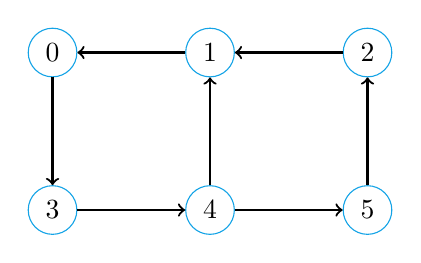
\begin{tikzpicture}
            \begin{scope}[every node/.style={circle, draw=Cerulean}]
                \node (0) at (0, 2) {$0$};
                \node (1) at (2, 2) {$1$};
                \node (2) at (4, 2) {$2$};
                \node (3) at (0, 0) {$3$};
                \node (4) at (2, 0) {$4$};
                \node (5) at (4, 0) {$5$};
            \end{scope}

            \begin{scope}[every edge/.style={thick, draw=black}]
                \draw (0) edge[->] (3);
                \draw (3) edge[->] (4);
                \draw (4) edge[->] (5);
                \draw (5) edge[->] (2);
                \draw (2) edge[->] (1);
                \draw (4) edge[->] (1);
                \draw (1) edge[->] (0);
            \end{scope}
        \end{tikzpicture}
    \end{figure}
\end{exmp}

\section{Eulerian Graph}

\begin{defn}
    In a graph $G$, a \emph{circuit} is a closed trail.
\end{defn}

\begin{defn}
    A simple graph $G$ is \emph{Eulerian} if it has a a circuit containing all edges.
\end{defn}

\begin{thm}
    A simple graph $G$ is Eulerian if and only if $G$ is both connected and every vertex has even degree.
\end{thm}

\begin{proof}
    Suppose $G$ contains a Eulerian circuit. Fix any vertex $v$ in the circuit, and for each incoming edge $(u, v)$ in the circuit, there must be an outgoing edge $(v, w)$. Since each edge is distinct, and $G$ is simple, each vertex adjacent to $v$ is used at most once. The degree of $v$ must be at least twice the number of times the circuit visits $v$. However, the circuit is Eulerian and so uses each edge \emph{exactly} twice, and so the degree of $v$ is even.

    Now, instead suppose that every vertex in $G$ has even degree, and $G$ is connected. We proceed by induction on $\abs{E(G)}$. Suppose $\abs{E(G)} = 3$, then we must have $K_3$ as a subgraph of $G$ and so provides an Eulerian circuit. Suppose now that such a circuit exists of $\abs{E(G)} \leq n-1$, and that we have a graph with $\abs{E(G)} = n$. Since $G$ is connected, there are no vertices of degree zero. Therefore, $\delta G \geq 2$, and so $G$ must contain a cycle $C$. Consider $E(G) \setminus E(C)$. Then each connected component of the resulting graph must still have vertices of even degree, and so by the induction hypothesis, each remaining component has an Eulerian cycle.
\end{proof}

\section{Extremal Graphs}

\begin{lemma}\label{lemma:listing}
    Let $G$ be an acyclic simple graph with $k$ connected components. Then $\abs{E(G)} - \abs{V(G)} + k = 0$.
\end{lemma}

\begin{proof}
    Each connected component $c_i$ with $n_i$ vertices must have $n_i-1$ edges. Therefore,
    \begin{align*}
        0 &= \sum_{i=1}^{k}\left(n_i - 1 - n_i + 1\right) = \sum_{i=1}^{k}\left(n_i-1\right) - \sum_{i=1}^{k}n_i + \sum_{i=1}^{k}1 \\
        &= \abs{E(G)} - \abs{V(G)} + k.
    \end{align*}
\end{proof}

\begin{prop}
    Every tree $T$ with at least two vertices must contain at least two vertices of degree equal to one. By Lemma \ref{lemma:listing}, $\abs{E(T)} = \abs{V(T)} - 1$. So $2\abs{E(T)} = 2\abs{V(T)} - 2$, and so $\sum_{v \in V(G)}deg(v) = 2\abs{V(T)} - 2$.
\end{prop}

\begin{thm}
    If $\abs{E(G)} > \left(\frac{\abs{V(G)}}{2}\right)^2$, then $K_3$ is a subgraph of $G$.
\end{thm}

\begin{proof}
    Suppose that $K_3$ is \emph{not} a subgraph of $G$. Notice that (for any simple graph) we have
    \begin{align*}
        \sum_{(u, v) \in E(G)}\left[deg(u) + deg(v)\right] = \sum_{v\in V(G)}deg(v)^2.
    \end{align*}
    Since $K_3$ is not a subgraph, any adjacent vertices $u$ and $v$ cannot have another adjacent vertex in common. By the pigeonhole principle, we must therefore have $deg(u) + deg(v) \leq \abs{V(G)}$, and so
    \begin{align*}
        \sum_{v\in V(G)}deg(v)^2 \leq \abs{V(G)}\abs{E(G)}.
    \end{align*}
    By Cauchy-Schwarz \ref{cauchy-schwarz-triangle} applied to a vector of vertex degrees and the vector $\vec{1}$, we also must have
    \begin{align*}
        \frac{\left(\sum_{u \in V(G)}deg(u)\right)^2}{\abs{V(G)}} \leq \sum_{u \in V(G)}deg(u)^2.
    \end{align*}
    Therefore, by Lemma \ref{sum-degrees-is-twice-edges}, it follows that
    \begin{align*}
        \frac{\left(2\abs{E(G)}\right)^2}{\abs{V(G)}} \leq \sum_{u \in V(G)}deg(u)^2 \leq \abs{V(G)}\abs{E(G)},
    \end{align*}
    and so we obtain
    \begin{align*}
        \abs{E(G)} \leq \left(\frac{\abs{V(G)}}{2}\right)^2.
    \end{align*}
\end{proof}

\begin{defn}
    The \emph{degree sequence} of a graph is an sequence containing the degree of each vertex in $G$ exactly once.
\end{defn}

\begin{thm}{Havel-Hakimi}\label{thm:degree-sequence}\proofbreak
    Let $d_i \in \N$ such that $d_0 \geq d_1 \geq \cdots \geq d_{n-1}$. This sequence can be realized as the degree sequence of some graph if and only if the (unsorted) sequence $d_{1}-1, d_{2}-1, \cdots, d_{d_0}-1, d_{d_0+1}, \cdots, d_{n-1}$ can also be realized.
\end{thm}

\begin{proof}
    Suppose this new sequence can be realized in a graph $G$. Then we can add a new vertex $v_0$ with edges to $v_1, \ldots, v_{d_0}$, and we have realized this degree sequence.

    Suppose instead that the original degree sequence can be realized in graphs $G_0,\ldots, G_k$. Choose $G$ which maximizes
    \begin{align*}
        \sum_{v \in N_G(v_0)}deg(v).
    \end{align*}
    If $v_0$, which has degree $d_0$, is not adjacent to the next $d_0$ largest vertices, there must be some vertices $s$ and $r$ such that $v_0$ is adjacent to $r$, \emph{not} adjacent to $s$, and $deg(s) > deg(r)$. Since $deg(s) > deg(r)$, there exists a vertex $l$ such that $s$ to adjacent to $l$ and not to $r$. Replace edges $(s, l)$ and $(v_0, r)$ with $(v_0, s)$ and $(l, r)$. This preserves the degree sequence, but now the sum of degrees of vertices adjacent o $v_0$ is strictly larger, because $deg(s) > deg(r)$. Since this sum has a maximum possible value, we can repeat this process only a finite number of times. Now $v_0$ is adjacent to all and only the $d_0$ with next largest degrees, and so removing $v_0$ and its edges necessarily produces a graph with degree sequence $d_{1}-1, d_{2}-1, \cdots, d_{d_0}-1, d_{d_0+1}, \cdots, d_{n-1}$.
\end{proof}

\section{Directed Graphs}

\begin{defn}
    In a directed graph (or \emph{digraph}), edges consist of an ordered pair of vertices $(u, v)$, such we have an edge from $u$ to $v$, but not necessarily the reverse. Additionally, we allow loop edges. We may have distinct edges $(u, v)$ and $(v, u)$, but still do not allow multiple edges in the same direction between the same vertex.
\end{defn}

\begin{defn}
    The adjacency matrix is $A(G)$ such that $A[u, v] = 1$ only when $(u, v) \in E(G)$, and zero otherwise.
\end{defn}

\begin{defn}
    We define the \emph{in-degree} and \emph{out-degree} of vertices to be the number of incoming directed edges, and outgoing directed edges respectively.
\end{defn}

\begin{defn}
    The \emph{complete digraph} on $n$ vertices has edges $(u, v), (v, u)$ for each pair of vertices $u$ and $v$, as well as all possible loop edges.
\end{defn}

\begin{defn}
    A \emph{functional graph} is a digraph where there exists a function $f: \Z_n \to \Z_n$ such that every edge has the form $(i, f(i))$. Given a function $f: \Z_n \to \Z_n$, we define $G_f$ to be the functional graph induced by this function.
\end{defn}

\begin{prop}
    Let $G_f$ be a functional digraph. If $f(\Z_n) = \Z_n$, then $G_f$ is a union of disjoint directed cycles. Alternatively, if $\abs{f^(n-1)(\Z_n)} = 1$ then the undirected form of $G_f$ is a tree.
\end{prop}

\begin{proof}
    Suppose $f(\Z_n) = \Z_n$, which implies $f$ is surjective and since $\abs{\Z_n} = \abs{\Z_n}$, we find that $f$ must be a bijection. Therefore, every vertex has exactly one incoming edge and one outgoing edge, and therefore must be the union of disjoint cycles.

    Suppose that $f^(n-1)(\Z_n) = \{r\}$. Therefore, in the undirected form of $G_f$, there is a path from $u$ to $r$, and $v$ to $r$ for any $u, v \in V(G_f)$, and so there is a path $u \sim \cdots \sim r \sim \cdots \sim v$, and so the graph is connected. Since there cannot be loop edges other than $f(r) = r$ (or else the vertex with the loop would be in $f^(n-1)(\Z_n)$), there are $n-1$ edges in the unidrected form of $G_f$. Since $G_f$ is connected and has $n-1$ edges, it is a tree by Theorem \ref{tree-edges-iff}.
\end{proof}

\begin{prop}
    The set of all functional graphs describing spanning unions of directed cycles in a graph $G$ is $\det(A_G)$, where $A_G$ is the symbolic adjacency matrix.
\end{prop}

\begin{proof}
    
\end{proof}

\begin{rmk}
    We can list of possible subgraphs of a directed graph $G$ as
    \begin{align*}
        \prod_{(u, v) \in E(G)}\left(a_{u,v}^{0} + a_{u,v}^{1}\right).
    \end{align*}
\end{rmk}

\begin{prop}
    The number of functional forests wih vertex set $\Z_n$ is at least $2(n!)-1$.
\end{prop}

\begin{proof}
    Given $f: \Z_n \to \Z_n$, if there exists a non-trivial cycle then there is some $i$, $j$, and $k$ such that $f(i) = j$, $f^(k)(j) =i$, and $i \neq j$. Therefore, if $f(i) \leq i$ for all $i \in \Z_n$ then all cycles are loop edges, and so $f$ describes a forest of functional trees.

    Consider the symbolic listing of such $f$. This is
    \begin{align}
        \sum_{f\in S_n,\forall i[f(i)\leq i]}\prod_{i \in \Z_i}a_{i,f(i)} = \prod_{i\in\Z_n}\left(\sum_{0\leq j \leq i}a_[ij]\right),
    \end{align}
    which is a polynomial with $n!$ terms.

    Similarly, $f$ such that $f(i) \geq i$ gives $n!$ functional forests. Since only the identity permutation is in both sets, the total size of this subset of functional forests is $2(n!) - 1$.
\end{proof}

\begin{defn}{Gantmacher Notation}\proofbreak
    Let $M$ be an $N\times n$ matrix and let $\{i_k\}, \{j_k\}$ be two subsequences of $0, 1, \ldots, n-1$ of the same length $l$. In Gantmacher notation,
    \begin{align*}
        M\begin{bmatrix}
            i_0, &i_1, &\ldots, &i_{l-1} \\
            j_0, &j_1, &\ldots, &j_{l-1} \\
        \end{bmatrix}
    \end{align*}
    is the $l\times l$ matrix obtained by \emph{retaining} only rows indexed by $i_k$ and columns indexed by $j_k$.
\end{defn}

\begin{exmp}
    Let $M$ be a generic $4 \times 4$ matrix with entries $M_{ij}$. Then
    \begin{align*}
        M\begin{bmatrix}
            0, &2, &3 \\ 1, &2, &3
        \end{bmatrix} = \begin{bmatrix}
            M_{01} & M_{02} & M_{03} \\
            M_{21} & M_{22} & M_{23} \\
            M_{31} & M_{32} & M_{33}
        \end{bmatrix}.
    \end{align*}
\end{exmp}

\begin{thm}{Sylvester's Identity or the generalized Cauchy-Binet formula}\proofbreak
    Let $A$ be a $p \times q$ and $B$ a $q \times p$ matrix. Let $[n]$ denote the set $\{1, \ldots, n\}$ and $\binom{[n]}{k}$ denote the set of all $\binom{n}{k}$ possible subsets of $[n]$ with $k$ elements. For some $k \leq p$, let $I, J \in \binom{[q]}{k}$, and then:
    \begin{align*}
        \det\left((AB)\begin{bmatrix}
            I \\ J
        \end{bmatrix}\right) = \sum_{K\in \binom{[q]}{k}}\det\left(A\begin{bmatrix}I \\ K\end{bmatrix}\right)\det\left(B\begin{bmatrix}K \\ J\end{bmatrix}\right),
    \end{align*}
    where $\binom{[q]}{k}$ is all possible subsets of $\{1, \ldots, q\}$ with $k$ elements.
\end{thm}

\begin{rmk}
    When $k = 1$, this reduces to the standard formula for matrix multiplication:
    \begin{align*}
        (AB)_{ij} = \sum_{1\leq k \leq q}A_{ik}B_{kj}.
    \end{align*}
    When $k = q$, this is the Cauchy-Binet formula, which states that
    \begin{align*}
        \det(AB) = \sum_{K\in \binom{[q]}{p}}\det\left(A\begin{bmatrix}[p] \\ K\end{bmatrix}\right)\det\left(B\begin{bmatrix}K \\ [p]\end{bmatrix}\right).
    \end{align*}
\end{rmk}

\begin{lemma}{Determinant-Sum}\label{lemma:determinant-sum}\proofbreak
    \begin{align*}
        \det(A + diag(\vec{x})) = \sum_{0 \leq k \leq n}\sum_{0 \leq i_0 < i_1 < \cdots < i_{k-1} < n}\det\left(A\begin{bmatrix}
            i_0, &\cdots, &i_{k-1} \\ i_0, &\cdots, &i_{k-1}
        \end{bmatrix}\right)\prod_{j \in \Z_n \setminus \{i_0, \ldots, i_{k-1}\}}x_j.
    \end{align*}
\end{lemma}

\begin{proof}
    Taking $M = A + diag(\vec{x})$, then by Leibniz's formula we have
    \begin{align*}
        \det(M) = \sum_{\sigma\in S_n}sgn(\sigma)\left[\prod_{\substack{i \in \Z_n \\ \sigma(i) \neq i}}M_{i,\sigma_i}\right]\left[\prod_{\substack{i \in \Z_n \\ \sigma(i) = i}}M_{i,\sigma_i}\right].
    \end{align*}
    Since $M_{i,\sigma(i)} = A_{ii} + x_i$ when $\sigma(i) = i$ and $M_{i,\sigma(i)} = A_{i,\sigma(i)}$ otherwise, we have
    \begin{align*}
        \det(M) = \sum_{\sigma\in S_n}sgn(\sigma)\left[\prod_{\substack{i \in \Z_n \\ \sigma(i) \neq i}}A_{i,\sigma(i)}\right]\left[\prod_{\substack{i \in \Z_n \\ \sigma(i) = i}}\left(A_{ii}+x_i\right)\right].
    \end{align*}
    Next, note that
    \begin{align*}
        \prod_{\substack{i \in \Z_n \\ \sigma(i) = i}}\left(A_{ii}+x_i\right) = \prod_{\substack{i \in \Z_n \\ \sigma(i) = i}}A_{ii} + \sum_{s\in S}\prod_{\substack{i \in \Z_n \\ \sigma(i) = i}}A_{ii}^{s_i}x_i^{1-s_i},
    \end{align*}
    where $S$ be the set of all binary sequences with one entry for each $i \in \Z_n$ such that $\sigma(i) = i$, and where at least one element of the sequence is zero.
    Therefore,
    \begin{align*}
        \det(M) &= \sum_{\sigma\in S_n}sgn(\sigma)\left[\prod_{\substack{i \in \Z_n \\ \sigma(i) \neq i}}A_{i,\sigma(i)}\right]\left[\prod_{\substack{i \in \Z_n \\ \sigma(i) = i}}A_{ii} + \sum_{s\in S}\prod_{\substack{i \in \Z_n \\ \sigma(i) = i}}A_{ii}^{s_i}x_i^{1-s_i}\right] \\
        &= \sum_{\sigma\in S_n}sgn(\sigma)\left[\prod_{i \in \Z_n}A_{i,\sigma(i)} + \prod_{\substack{i \in \Z_n \\ \sigma(i) \neq i}}A_{i,\sigma(i)}\sum_{s\in S}\prod_{\substack{i \in \Z_n \\ \sigma(i) = i}}A_{ii}^{s_i}x_i^{1-s_i}\right] \\
        &= \sum_{\sigma\in S_n}sgn(\sigma)\left[\prod_{i \in \Z_n}A_{i,\sigma(i)} + \prod_{\substack{i \in \Z_n \\ \sigma(i) \neq i}}A_{i,\sigma(i)}\sum_{s\in S}\prod_{\substack{i \in \Z_n \\ \sigma(i) = i}}A_{ii}^{s_i}x_i^{1-s_i}\right].
    \end{align*}
\end{proof}

\begin{thm}{Tutte's Directed Matrix Tree Theorem}\label{thm:directed-matrix-tree}
    Let $G$ is a directed graph, potentially with loop edges. A symbolic listing of all spanning subtrees is
    \begin{align*}
        \sum_{i\in\Z_n}A_{ii}\det\left(\left(diag(A_G\vec{1})-A_G\right)\begin{bmatrix}
            0, &\ldots, &i-1, &i+1, &\ldots, &n-1 \\
            0, &\ldots, &i-1, &i+1, &\ldots, &n-1.
        \end{bmatrix}\right),
    \end{align*}
    where each term in the sum lists all spanning subtrees rooted at vertex $i$.
\end{thm}

\begin{proof}
    A symbolic listing of spanning subtrees is given by
    \begin{align*}
        \sum_{\substack{f: \Z_n \to \Z_n \\ \abs{f^{n-1}(\Z_n)} = 1}}\prod_{i\in\Z_n}A_{i,f(i)}.
    \end{align*}
    Consider $A_{\mathit{IK}_{n+1}}$, where $\mathit{IK}_{n+1}$ is the complete directed graph. The listing of all functional trees on $n+1$ vertices, rooted at $n$, is
    \begin{align*}
        \sum_{\substack{f \in \Z_{n+1}\to\Z_{n+1} \\
        f^{(n)}(\Z_n) = \{n\}}}\prod_{i\in\Z_n}A_{i,f(i)} = A_{n,n}\det\left(-A_{\mathit{IK}_n} + diag(\vec{t})\right),
    \end{align*}
    where $\vec{t} \in \Z^{n}$ is defined by $t[u] = \sum_{v \in \Z_{n+1}}A_{u,v}$. By the Determinant-Sum Lemma, this is equal to
    \begin{align*}
        A_{n,n}\sum_{k\in\Z_n}\sum_{0 \leq i_0 < \cdots < i_{k-1}<n}\left(-1\right)^{k}\det\left(A_{\mathit{IK}_n}\begin{bmatrix}
            i_0, &\ldots, &i_{k-1} \\
            i_0, &\ldots, &i_{k-1}
        \end{bmatrix}\right)\prod_{u\in\Z_n\setminus \{i_0, \ldots, i_{k-1}\}}\vec{t}[u].
    \end{align*}
    Leibniz's formula gives us
    \begin{align*}
        \left(-1\right)^{k}\det\left(A_{\mathit{IK}_n}\begin{bmatrix}
            i_0, &\ldots, &i_{k-1} \\
            i_0, &\ldots, &i_{k-1}
        \end{bmatrix}\right) = \left(-1\right)^{k}\sum_{\sigma\in S_k}\left(-1\right)^{k-cycles(\sigma)}\prod_{j\in\Z_k}A_{i,\sigma(i)}.
    \end{align*}
    Since $(-1)^{k}(-1)^{k-cycles(\sigma)} = (-1)^{cycles(\sigma)}$, we have
    \begin{align*}
        \sum_{\sigma\in S_k}\left(-1\right)^{cycles(\sigma)}\prod_{j\in\Z_k}A_{i,\sigma(i)}.
    \end{align*}
    Applying product-sum exchange, we also have
    \begin{align*}
        \prod_{u\in\Z_n\setminus \{i_0, \ldots, i_{k-1}\}}\vec{t}[u] &= \prod_{u\in\Z_n\setminus \{i_0, \ldots, i_{k-1}\}}\sum_{v \in \Z_{n+1}}A_{u,v} = \sum_{f:\Z_n\to\Z_{n}\setminus\{i_0, \ldots, i_{k-1}\}}\prod_{u\in\Z_n\setminus\{i_0, \ldots, i_{k-1}\}}A_{u,f(u)}.
    \end{align*}
    Therefore, assembling these pieces produces
    \begin{align*}
        A_{n,n}\sum_{k\in\Z_n}\sum_{0 \leq i_0 < \cdots < i_{k-1}<n}\sum_{\sigma\in S_k}\left(-1\right)^{cycles(\sigma)}\prod_{j\in\Z_k}A_{i,\sigma(i)}\sum_{f:\Z_n\to\Z_{n}\setminus\{i_0, \ldots, i_{k-1}\}}\prod_{u\in\Z_n\setminus\{i_0, \ldots, i_{k-1}\}}A_{u,f(u)}.
    \end{align*}
    Rearranging, we therefore obtain
    \begin{align*}
        \sum_{k\in\Z_n}\sum_{0 \leq i_0 < \cdots < i_{k-1}<n}\sum_{f:\Z_n\to\Z_{n}\setminus\{i_0, \ldots, i_{k-1}\}}\sum_{\sigma\in S_k}\left(-1\right)^{cycles(\sigma)}A_{n,n}\prod_{j\in\Z_k}A_{i,\sigma(i)}\prod_{u\in\Z_n\setminus\{i_0, \ldots, i_{k-1}\}}A_{u,f(u)}.
    \end{align*}
    Since product of $A_{n,n}$ and the two products produces a symbolic functional graph on $n+1$ vertices, with a loop edge at $n$, a spanning union of disjoint cycles on $\{i_0, \ldots, i_{k-1}\}$, and an arbitrary functional component on the remaining vertices.

    Next, we utilize Zeilberger pairing. We want to bijections between these functional graphs that prove graphs with cycles will cancel out. Among all possible cycles in the graph, if any cycles exist let $v_0$ be the smallest vertex appearing in any cycle. We then pair the graph with a \emph{conjugate graph} with the same vertex and edge set, but now we color the cycle contain $v_0$ oppositely --- that is, we move it between the two products while leaving the graph itself unchanged. Since this changes the number of cycles in $\sigma$ by one, the sign of $(-1)^{cycles(\sigma)}$ flips, and so all graphs with any cycles cancel out with their pair.
\end{proof}

\begin{cor}{Cayley's formula}\label{cor:cayley-formula}\proofbreak
    There are $n^{n-1}$ directed functional spanning subtrees of $K_{n}$.
\end{cor}

\begin{proof}
    By Tutte's Directed Matrix-Three Theorem, the number of such trees is
    \begin{align*}
        \sum_{i\in\Z_n}K_{ii}\det\left(diag(K_n\vec{1}) - K_n\right)\begin{bmatrix}
            0, &\ldots, &i-1, &i+1, &\ldots, &n-1 \\
            0, &\ldots, &i-1, &i+1, &\ldots, &n-1.
        \end{bmatrix}
    \end{align*}
    Since all terms of this sum are the same, we have that the number of such trees is
    \begin{align*}
        n\det(nI_{n-1}-K_{n-1}).
    \end{align*}
    Since $nI_{n-1} - K_{n-1}$ is a polynomial of $K_{n-1}$, its eigenvalues are $1$ with multiplicity one, and $n$ with multiplicity $(n-1)-1$. Therefore, the count of trees is $n\cdot 1 \cdot n^{n-2} = n^{n-1}$.
\end{proof}

\begin{cor}
    Let $d_0, \ldots, d_{n-1}$ be a \emph{in-degree} sequence. The number of spanning subtrees of the complete directed graph on $n$ vertices, such that the subtrees have this in-degree sequence, is given by
    \begin{align*}
        \binom{n-2}{d_0, \ldots, d_{i-1}, d_{i}-2, d_{i+1}, \ldots, d_{n-1}},
    \end{align*}
    where $i$ is the root of the directed tree.
\end{cor}

\begin{cor}
    Let $A$ be an adjacency matrix, where we instantiate $A[i,j]$ with the product of the in-degree and out-degree of vertices $i$ and $j$ respectively. Therefore $A = xy^{\transpose}$, where $x_i$ the the in-degree of vertex $i$ and $y_j$ is the out-degree of vertex $j$.

    By Tutte's Theorem \ref{thm:directed-matrix-tree}, the number of directed spanning subtrees rooted at vertex $i$ is listed by
    \begin{align*}
        A_{ii}\det\left(diag(A\vec{1}) - A\right)\begin{bmatrix}
            0, &\ldots, &i-1, &i+1, &\ldots, &n-1 \\
            0, &\ldots, &i-1, &i+1, &\ldots, &n-1.
        \end{bmatrix} = x_iy_i\det\left[diag(x)\left(\left[\sum_{0\leq < n}y_i\right]I_{n-1} - \vec{1}y^{\transpose}\right)\right]
    \end{align*}
    Given the structure of $A$, we obtain the following listing of trees rooted at $i$:
    \begin{align*}
        \left(\prod_{j\in\Z_n}x_j\right)y_i^2\left(\sum_{j\in\Z_n}y_i\right)^{n-2}.
    \end{align*}
    Therefore, the count we are looking for is the number of terms in the expanded form of $\left(\sum_{j\in\Z_n}y_i\right)^{n-2}$ which are $y_0^{d_0} + y_1^{d_1} + \cdots + y_i^{d_i-2} + \cdots + y_n^{d_n}$, where the $d_i-2$ comes from the fact we have $y_i^2$ on the outside. The number of such terms, and therefore our count, is given by the multinomial coefficient
    \begin{align*}
        \binom{n-2}{d_0, \ldots, d_{i-1}, d_{i}-2, d_{i+1}, \ldots, d_{n-1}}.
    \end{align*}
\end{cor}

\begin{defn}
    An \emph{orientation graph} $G$ is a subgraph of $\mathbb{K}_n$ such that precisely one of $(i, j)$ or $(j, i)$ is included in $V(G)$ for all $0 \leq i, j < n$.
\end{defn}

\begin{defn}
    Consider a graph $G$, where each vertices corresponds to a position on the unit circle in $\C$ such that vertex $u$ will be placed at $\exp\left(2\pi i\frac{u}{n}\right)$. For any subgraph $G_0$, define $G_k$ for $0 \leq k < \frac{n}{\abs{V(G_0)}}$ by
    \begin{align*}
        V(G_k) = \left\{\exp\left(2\pi i\frac{k}{n}\right)v \compbar v \in V(G_0)\right\}.
    \end{align*}
    We say that this is a \emph{cyclic decomposition} if $G$ is an orientation of $\mathbb{K}_n$ and the $G_k$ give a decomposition of $G$.
\end{defn}

\begin{defn}
    A graph $G_f$ is gracefully labeled if $\left\{\abs{f(i) - i} : i \in \Z_n\right\} = \Z_n$. A graph is graceful if it admits a graceful labeling --- that is, there exists $\sigma \in S_n$ such that $i \mapsto \sigma(i)$ and $f(i) \mapsto \sigma(f(i))$ gives a graceful labeling.
\end{defn}

\begin{thm}{Rosa's Theorem}\label{thm:rosas}\proofbreak
    An orientation of $\mathbb{K}_{2n-1}$ admits a cyclic decomposition generated by a functional graph $G_f$ if and only if $G_f$ is graceful.
\end{thm}

\begin{proof}
    Suppose that $G_f$ is gracefully labeled, then
    \begin{align*}
        \bigunion_{k\in\Z_{n-1}}\omega^{k}G_f
    \end{align*}
    yields such a decomposition.

    Suppose that $G_f$ is not graceful, so for all $\sigma\in S_n$, the graphs $\omega^{k}G_{\sigma f \sigma^{-1}}$ will not be edge disjoint for all $\omega$.
\end{proof}

\begin{thm}{Kotzig-Ringel Rosa Conjecture}\label{thm:graceful-labeling}
    If $G_f$ is an $n$-vertex functional tree, then an orientation of $\mathbb{K}_{2n-1}$ admits a cycle decomposition into $2n-1$ subgraphs cyclically generated by $G_f$.
\end{thm}

\section{Matching}

\begin{defn}
    Given an undirected simple graph $G$, a \emph{matching} $M$ of $G$ is a non-empty subset $S \subseteq E(G)$ such that no edges in $S$ have a common endpoint.
\end{defn}

\begin{defn}
    A matching $M$ is perfect when $\abs{M} = \abs{V(G)}/2$.
\end{defn}

\begin{prop}
    There are $\frac{(2n)!}{2^{n}n!}$ perfect matching in $K_{2n}$.
\end{prop}

\begin{defn}
    Let $G$ be a graph, and let Tutte's Skew Symmetric Matrix $T_G$ be the matrix where
    \begin{align*}
        T_g[u, v] &= \begin{dcases}
            0, &\{u, v\} \not\in E(G), \\
            a_{u,v}, &\{u, v\} \in E(G) \land u < v, \\
            -a_{v, u}, &\{u, v\} \in E(G) \land u > v
        \end{dcases}.
    \end{align*}
\end{defn}

\begin{lemma}\label{lemma:tutte-odd-cycle-cancellation}
    Let $O \subseteq S_n$ be all permutations $f$ such that $G_f$ contains at least one odd cycle. For any graph $G$, the polynomial
    \begin{align*}
        \sum_{\sigma\in O}sgn(\sigma)\prod_{i\in\Z_n}T_G\left[i,\sigma(i)\right]
    \end{align*}
    is identically zero.
\end{lemma}

\begin{proof}
    If $\sigma \in O$ contains a fixed point $i = \sigma(i)$, then the corresponding term in the polynomial is a product containing the term $T_G[i,i] = 0$, and so those terms vanish.

    We now pair the remaining permutations and show each pair cancels with each other. For each odd cycle, let $i$ be the smallest vertex and label the cycle $i\sigma(i)\sigma^(2)(i)\cdots$ with the string of it's vertices in the order they appear in the cycle. Let $C_{\sigma}$ be the largest odd-cycle in $G_{\sigma}$, taking the one containing the smallest vertex if there are multiple equally large odd-cycles.

    We pair the permutation $\sigma$ with $\sigma^{*}$, where $\sigma$ and $\sigma^{*}$ are the same except the largest cycle has been reversed. Since $C_{\sigma}$ is odd, $C_{\sigma^{*}}$ is odd, so $\sigma^{*} \in O$. Therefore, this is indeed a pairing.

    Furthermore, $sgn(\sigma) = sgn(\sigma^{*})$, and also
    \begin{align*}
        \prod_{i\in\Z_n}T_{G}\left[i,\sigma(i)\right] = -\prod_{i\in\Z_n}T_{G}\left[i,\sigma^{*}(i)\right],
    \end{align*}
    since the products are identical except for the sign of the edge variables corresponding to $C_{\sigma}$ and $C_{\sigma^{*}}$. Since these cycles are odd, the products differ by a sign, and so the corresponding terms in the polynomial must indeed cancel each other.
\end{proof}

\begin{thm}{Tutte's Matching Theorem}\label{thm:tutte-matching}\proofbreak
    A simple undirected graph $G$ contains a perfect matching if and only if the determinant of $T_G$ is not the zero polynomial.
\end{thm}

\begin{proof}
    We know that
    \begin{align*}
        \det(T_G) &= \sum_{\sigma\in S_n}sgn(\sigma)\prod_{i\in\Z_n}T_G[i,\sigma(i)] \\
        &= \sum_{\sigma\in O}sgn(\sigma)\prod_{i\in\Z_n}T_G[i,\sigma(i)] + \sum_{\sigma\in S_n\setminus O}sgn(\sigma)\prod_{i\in\Z_n}T_G[i,\sigma(i)] \\
        &= 0 + \sum_{\sigma\in S_n\setminus O}sgn(\sigma)\prod_{i\in\Z_n}T_G[i,\sigma(i)]
    \end{align*}
    by the Leibniz formula and Lemma \ref{lemma:tutte-odd-cycle-cancellation}.

    Note that $S_n\setminus O$ is the set of permutations containing only even cycles. Therefore, if $\det(T_G)$ is non-zero then there must exist at least one $\sigma \in S_n\setminus O$ which is a spanning union of even cycles. Any even cycle is a matching on its vertices, so then $G$ would have a perfect matching.

    Suppose that $G$ has a perfect matching
    \begin{align*}
        M = \left\{(u_1, v_1), (u_2, v_2), \ldots, (u_{\frac{n}{n}}, v_{\frac{n}{n}})\right\}.
    \end{align*}
    For the sake of simplicity, assume we have listed the matching such that $u_i < v_i$.

    Therefore, there is $\gamma \in S_n\setminus O$ which describes this matching as a spanning union of two-cycles, such that every edge $(u_i, v_i)$ in the matching corresponds to the two-cycle $u_i \sim v_i \sim u_i$. Therefore, the Leibniz formula of $\det(T_G)$ must contain the term
    \begin{align*}
        sgn(\gamma)\prod_{1\leq i\leq\frac{n}{2}}\left(A_{u_i,v_i}\right)\left(-A_{u_i,v_i}\right) = sgn(\gamma)\left(-1\right)^{\frac{n}{2}}\prod_{1\leq i\leq\frac{n}{2}}\left(A_{u_i,v_i}\right)^2.
    \end{align*}
    Any other term in the Leibniz formula of $T_G$ with the exact same edges must have the same sign, since changing the orientation of edges in a two-cycle does not change it's sign. Therefore, no terms can cancel with the term corresponding to $\gamma$, and so $\det(T_G)$ cannot be zero.
\end{proof}

\begin{defn}
    Given a graph $G$ and a matching $M$, a vertex $v \in V(G)$ is \emph{$M$-unsaturated} if no edge in $M$ is incident to $v$.
\end{defn}

\begin{defn}
    Given a graph $G$ and a matching $M$, a path $P$ is an \emph{$M$-alternating} path if edges of $P$ successively alternate between $M$ and $E(G) \setminus M$.
\end{defn}

\begin{defn}
    Given a graph $G$ and a matching $M$, a path $P$ in $G$ is an \emph{augmenting} path if it is $M$-alternating and the endpoints are both $M$-unsaturated.
\end{defn}

\begin{lemma}\label{lemma:matching-symmetric-difference}
    Let $M$ and $M'$ both be matchings in a graph $G$ and consider their symmetric difference $M \triangle M'$. The non-trivial connected components of $M \triangle M'$ are paths and even cycles.
\end{lemma}

\begin{proof}
    Let $H = M \triangle M'$, and notice that every $v \in H$ is adjacent to at most two edges. This is because $M$ cannot contain two edges incident to $v$, and neither can $M'$, so $H$ contains at most one edge from each that is adjacent to $v$.
\end{proof}

\begin{thm}{Berge's Theorem}\label{thm:berge-matching}\proofbreak
    Given a graph $G$, a matching $M$ is maximum if and only if $G$ has no $M$-augmenting path.
\end{thm}

\begin{proof}
    If $G$ has an $M$-augmenting path $P$, then we could increase the size of $M$ by swapping every edge in $P$ in or out of $M$, and so $M$ could not be maximum.

    If $M$ is not maximum, there exists some larger matching $M'$, and so by Lemma \ref{lemma:matching-symmetric-difference} we know the connected components of $M \triangle M'$ are even cycles or paths. Since an even cycle in $M \triangle M'$ contains an equal number of edges of $M$ and $M'$, there must be a path $P$ in $M \triangle M'$. However, such a path is necessarily an augmenting path in $M$.
\end{proof}

\begin{thm}{Hall's Theorem}
    Let $G$ be a bipartite graph with parts $U$ and $W$. THere exists a matching $M$ which saturates $U$ if and only if, for every $S \subseteq U$, we have $\abs{S} \leq \abs{N(S)}$.
\end{thm}

\begin{proof}
    If $\abs{N(S)} < \abs{S}$ for some $S \subseteq U$, we clearly cannot saturate $S$ with any matching $M$.

    Suppose for the sake of contradiction that Hall's condition holds yet no matching saturates $U$. Then take $M$ to be any maximum matching. Since $M$ does not saturate $U$, there exist some vertex $u \in U$ not saturated by $M$. Let $P$ be any $M$-alternating with endpoint $u$ (at least one trivially exists by taking a single edge to be the path), and let $S$ be the set of all vertices in the path. Since $M$ is assumed to be maximum, by Berge's theorem \ref{thm:berge-matching} $u$ is the only unsaturated vertex in $S$. Now define $U' = U \intersection S$ and $W' = W \intersection S$, so $W'$ and $U' \setminus \{u\}$ are both saturated. Since $G$ is bipartite, it must be that $\abs{W'} = \abs{U'} - 1$. Therefore, $W' \subseteq N(U')$.

    Now we show by contradiction that for any $w \in N(U')$, there is a $u,w$ $M$-alternating path.
\end{proof}

\begin{cor}
    Every regular bipartite graph with parts $U$ and $V$ must have $\abs{U} = \abs{V}$ and has a perfect matching.
\end{cor}

\begin{cor}
    For $A \in \R_{\geq 0}^{n\times n}$, then $\perm(A) = 0$ if and only if $PAP^{\transpose}$ does not contain an $r \times c$ zero block, where $c + r \geq n$ and $P$ is a permutation matrix.
\end{cor}
